\documentclass[openright,letterpaper,12pt]{book}
\usepackage[utf8]{inputenc}
\usepackage[french]{babel}
\usepackage{graphicx}
\usepackage{float}
\usepackage{pdfpages}
\usepackage[plainheadsepline,markcase=ignoreuppercase]{scrlayer-scrpage}
\usepackage{titlesec}
\usepackage{tocloft}
\usepackage{hyperref}
\usepackage{geometry}
\usepackage{listings}
\usepackage[dvipsnames]{xcolor}
\hypersetup{
		pdfauthor={Alexandre Dumont},
		pdftitle={MegaYoko},
		pdfsubject={Guide d'utilisateur},
		pdfkeywords={Manuel},
		%pdftex,
		colorlinks=true,
		breaklinks=true,
		urlcolor=RoyalBlue,
		linkcolor=RoyalBlue,
		citecolor=RoyalBlue,
		bookmarksopen=true,
		unicode=true
}
\usepackage{bookmark}
\usepackage{cmap} % Doit
\usepackage[T1]{fontenc}
\usepackage[hyperpageref]{backref}

\geometry{letterpaper, inner=1.5in, outer=1.0in, tmargin=1.5in, bmargin=1.0in, twoside=false}

\pagestyle{scrheadings}
%\renewcommand{\chaptermark}[1]{\markboth{{\thechapter. #1}}{}}
%\renewcommand{\sectionmark}[1]{aa}
\setlength{\headheight}{18pt}
\setlength{\footheight}{18pt}

\definecolor{codegreen}{rgb}{0,0.6,0}
\definecolor{codegray}{rgb}{0.5,0.5,0.5}
\definecolor{codepurple}{rgb}{0.58,0,0.82}
\definecolor{backcolour}{rgb}{1,1,1}

\lstdefinestyle{mystyle}{
	emph={get, output\_en, level},
    backgroundcolor=\color{backcolour},   
    commentstyle=\color{codegreen},
    keywordstyle=\color{codegreen},
    emphstyle=\color{codegreen},
    numberstyle=\small\color{codegray},
    stringstyle=\color{codepurple},
    basicstyle=\ttfamily\large,
    breakatwhitespace=false,         
    breaklines=true,                 
    captionpos=b,                    
    keepspaces=true,                 
    numbers=left,                    
    numbersep=5pt,                  
    showspaces=false,                
    showstringspaces=false,
    showtabs=false,                  
    tabsize=2,
}

\lstset{style=mystyle}

\begin{document}
\pagenumbering{gobble}
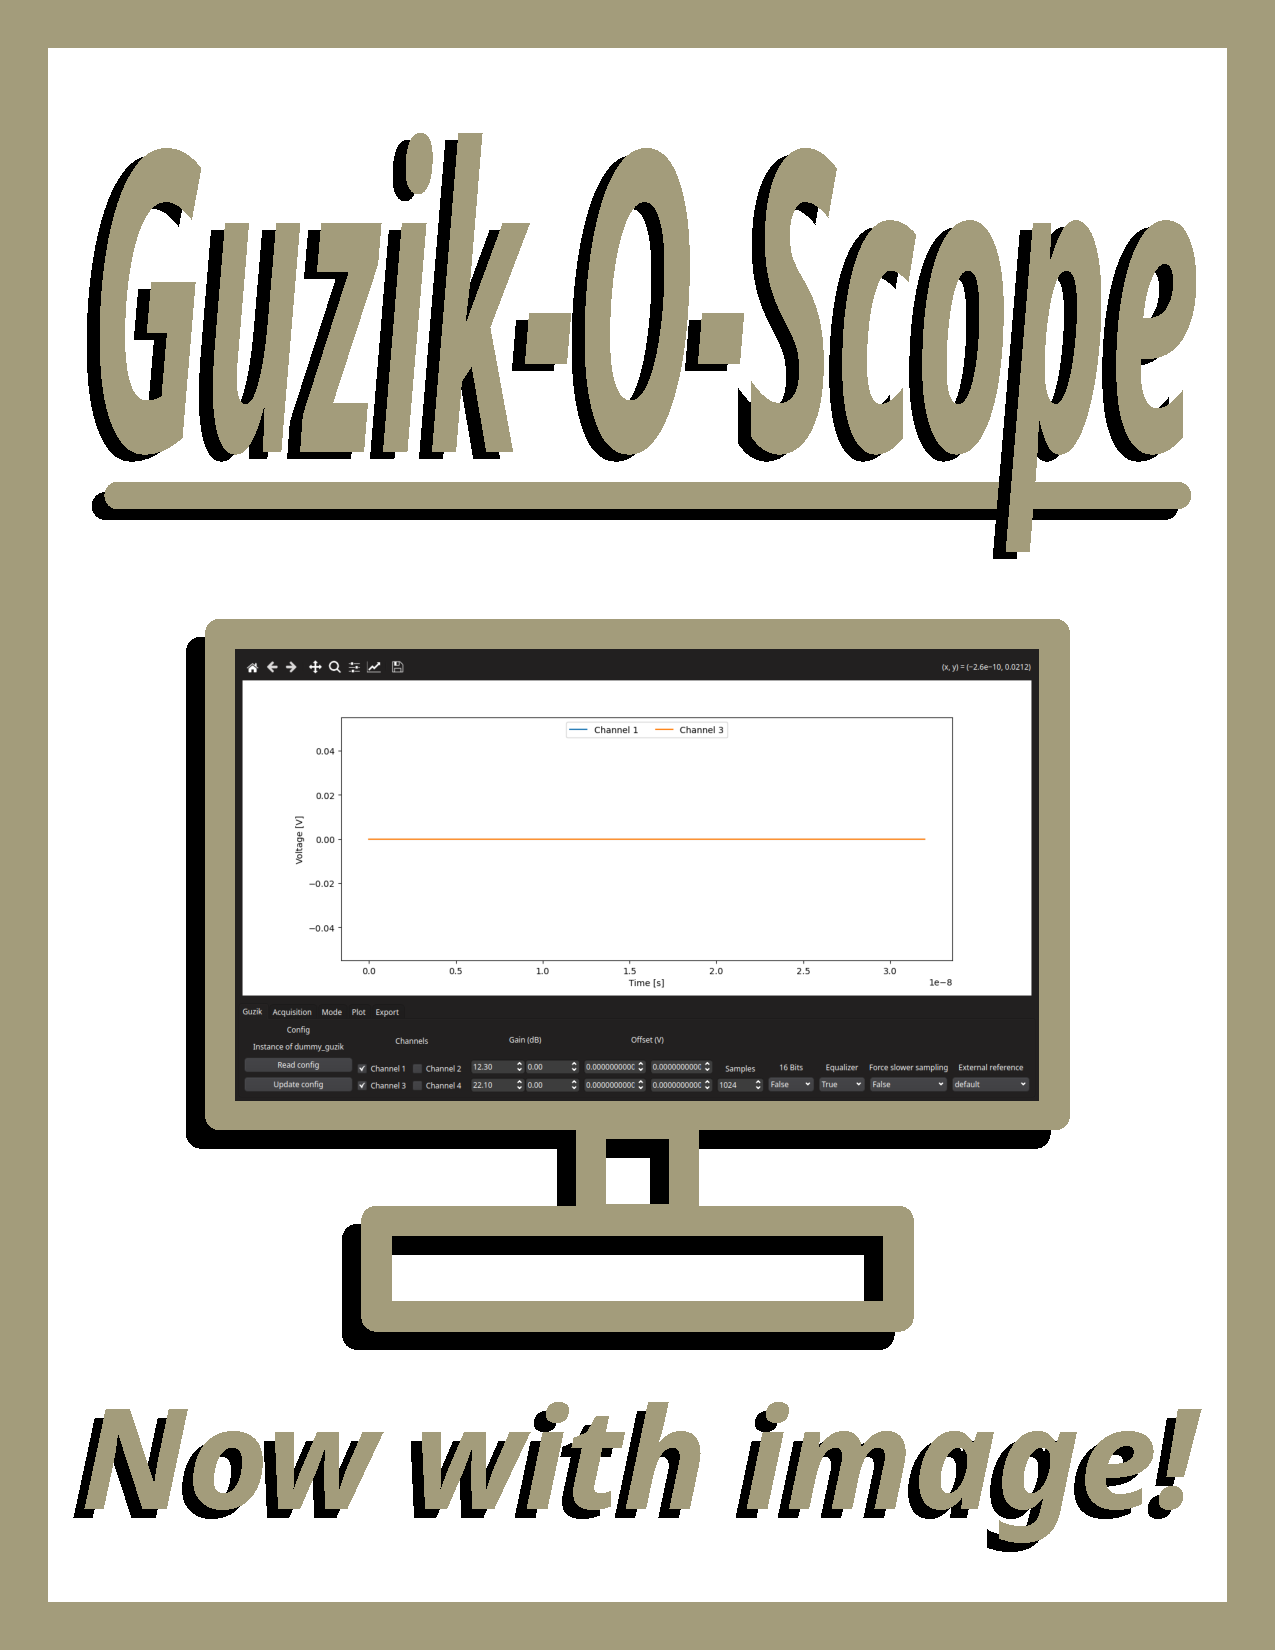
\includepdf[noautoscale=true, scale=1]{Figures/Pagetitre/pagetitre.pdf}
\clearpage\null\thispagestyle{empty}\clearpage
\thispagestyle{empty}
{\ } 

\vspace{3cm}
\noindent
{\fontsize{35.83pt}{40pt}\selectfont\bf Guzik-O-Scope\\} 
{\Large\bf Guide de l'utilisateur}

\vspace{10cm}\noindent
{\huge\bf Alexandre Dumont}\\
{\large ReuletLab}

\clearpage\null\thispagestyle{empty}

\renewcommand{\tableofcontents}
             {
                \clearpage
                \chapter*{\pdfbookmark[chapter]{\contentsname}{toc}
                          \contentsname}
                \csname @starttoc\endcsname{toc}
             }
\frontmatter
\chapter*{Garantie}
\addcontentsline{toc}{chapter}{Garantie}
Les instructions, le code et ce manuel sont fournis sans garanties et sans 
support et peuvent ne pas fonctionner.
\clearpage\null\thispagestyle{empty}

\tableofcontents
\clearpage\null\thispagestyle{empty}

\mainmatter

\clearpage
\chapter*{Utilisation}
\addcontentsline{toc}{chapter}{Utilisation}

\section*{Chargement du code pyHegel}
\addcontentsline{toc}{section}{Chargement du code pyHegel}
Pour pouvoir utiliser MegaYoko, il faut charger le code qui définit 
l'instrument pyHegel. 
Pour se faire, simplement ouvrir une console pyHegel et exécuter la commande
\begin{lstlisting}[]
%run -i MegaYoko.py
\end{lstlisting}
Pour utiliser MegaYoko dans un script, il faut plutôt utiliser la commande 
\verb+import+ de python,
\begin{lstlisting}[language=Python]
from MegaYoko.py import MegaYoko
\end{lstlisting}

\lstset{emph={MegaYoko,get,set,level,range,output_\en}}

\section*{Initialisation}
\addcontentsline{toc}{section}{Initialisation}
Une fois le code exécuté, la classe \verb+MegaYoko+ devient accessible. 
Pour l'initialiser, il faut charger deux sources individuelles et appeler le 
constructeur de la classe \verb+MegaYoko+.
\begin{lstlisting}[language=Python]
;load yo1
;load yo2

megaYoko = MegaYoko(yo1,yo2)
\end{lstlisting}

\section*{Paramètres}
Les différents paramètres accessibles de MegaYoko sont tous analogues aux 
paramètres des sources individuelles. 
Ceci permet donc d'utiliser MegaYoko à la place d'une source seule avec des 
modifications minimales aux scripts d'acquisition des données déjà existants. 
Les sous-sections suivantes seront dédiées à chacun des paramètres actuellement 
implémentés.
\addcontentsline{toc}{section}{Paramètres}

\subsection*{level}
\addcontentsline{toc}{subsection}{level}
Tout comme le paramètre \verb+level+ d'une source Yokogawa seule, celui-ci 
dicte la tension appliquée en sortie. 
Ce paramètre peut être lu en utilisant la commande \verb+get+,
\begin{lstlisting}[language=Python]
get(megaYoko.level)
\end{lstlisting}
et peut être modifié en utilisant plutôt la commande \verb+set+
\begin{lstlisting}[language=Python]
set(megaYoko.level, valeur)
\end{lstlisting}
où \verb+valeur+ doit être un nombre. 

\vspace{0.5cm}
Lorsque ce paramètre est modifié, la classe fait des calculs à l'interne pour 
déterminer quelle partie de la tension doit être appliquée par chacune des 
sources. 
Pour assurer le bon fonctionnement de MegaYoko ainsi que l'exactitude de ces 
calculs, il est impératif de respecter les branchements indiqués dans le 
chapitre précédent.

\subsection*{range}
\addcontentsline{toc}{subsection}{range}
Tout comme le paramètre \verb+range+ d'une source Yokogawa seule, celui-ci sert 
à définir l'échelle de tension de la source. 
Contrairement à une source seule, ce paramètre est maintenant une liste qui 
doit contenir deux valeurs.
Ce paramètre peut être lu en utilisant la commande \verb+get+,
\begin{lstlisting}[language=Python]
get(megaYoko.range)
\end{lstlisting}
et peut être modifié en utilisant plutôt la commande \verb+set+
\begin{lstlisting}[language=Python]
set(megaYoko.range, [valeur1, valeur2])
\end{lstlisting}
où \verb+valeur1+ et \verb+valeur2+ doivent être des nombres. 

\subsection*{output\_en}
\addcontentsline{toc}{subsection}{output\_en}
Le paramètre \verb+output_en+ détermine si la sortie est active ou non.
Ce paramètre peut être lu en utilisant la commande \verb+get+,
\begin{lstlisting}[language=Python]
get(megaYoko.output_en)
\end{lstlisting}
et peut être modifié en utilisant plutôt la commande \verb+set+
\begin{lstlisting}[language=Python]
set(megaYoko.output_en, valeur)
\end{lstlisting}
où \verb+valeur+ doit être une variable booléenne, soit \verb+True+ ou 
\verb+False+ ou encore 1 ou 0.
\clearpage\null\thispagestyle{empty}

\end{document}
